\chapter{Etude technique}
\usetikzlibrary{positioning} 
\usetikzlibrary{calc} 
\begin{spacing}{1.2}
\minitoc
\thispagestyle{MyStyle}
\end{spacing}
\newpage

\section*{Introduction}

\noindent Après avoir présenté le cadre général de notre projet, nous présenterons l'étude technique de notre projet dans laquelle nous commencerons par une description de l'environnement de développement de l'application en détaillant les technologies et frameworks utilisés. Finalement, nous présenterons l'architecture de notre système.

\section{Environnement de développement}

\noindent Cette section est consacrée à la présentation de l'environnement matériel et logiciel utilisé lors du développement de ce travail.

\subsection{Environnement matériel}

\noindent Ce travail a été réalisé avec un ordinateur ayant les caractéristiques suivantes :
\begin{itemize}
    \item Processeur : AMD Ryzen™ 7 3700U 2.30 GHz
    \item Mémoire : 12 Go
    \item Système d'exploitation : Windows 10
    \item Disque dur : 512 GB (SSD)
\end{itemize}

\subsection{Environnement logiciel}

\noindent Dans cette section, nous présentons les environnements logiciels utilisés pour le projet.

\subsubsection{Visual Studio Code}

\begin{figure}[H]%
    \center%
    {
        
\includegraphics[width=6cm,height=3cm]{images/vscode.png}%
    }
    \caption{Logo Visual Studio Code}%
\end{figure}

\noindent Visual Studio Code \cite{vscode} est un éditeur de code source développé par Microsoft. Dans notre projet, nous l'avons utilisé pour le développement de l'interface utilisateur React \cite{react} grâce à ses extensions avancées pour JavaScript et TypeScript \cite{typescript}.

\subsubsection{Visual Studio}

\begin{figure}[H]%
    \center%
    {
        
\includegraphics[width=6cm,height=2cm]{images/visualstudio.png}%
    }
    \caption{Logo Visual Studio}%
\end{figure}

\noindent Visual Studio \cite{visualstudio} est un environnement de développement intégré (IDE) de Microsoft. Nous l'avons utilisé pour développer notre API backend en .NET Core \cite{dotnet}, bénéficiant de ses outils de débogage et de gestion des packages NuGet.

\subsection{Technologies}

\noindent Dans cette section, nous présentons les langages de programmation, bibliothèques et frameworks utilisés pour le projet.

\subsubsection{Langages de programmation}

\noindent Nous commencerons par présenter les langages de programmation que nous avons utilisés pour réaliser ce projet.

\paragraph{TypeScript}

\begin{figure}[H]
    \centering
    
\includegraphics[width=3cm, height=3cm]{images/typescript.png}
    \caption{Logo TypeScript}
\end{figure}

\noindent TypeScript est un sur-ensemble typé de JavaScript qui compile vers du JavaScript simple. Dans notre projet, nous l'avons utilisé pour développer les composants React, apportant une meilleure détection d'erreurs et une meilleure maintenabilité du code frontend.

\paragraph{C\#}

\begin{figure}[H]
    \centering
    
\includegraphics[width=3cm, height=3cm]{images/csharp.png}
    \caption{Logo C\#}
\end{figure}

\noindent C\# est un langage de programmation orienté objet développé par Microsoft. Nous l'avons utilisé pour implémenter la logique métier de notre API .NET, gérant les opérations CRUD et la logique d'authentification.

\paragraph{Python}

\begin{figure}[H]
    \centering
    
\includegraphics[width=3cm, height=3cm]{images/python.png}
    \caption{Logo Python}
\end{figure}

\noindent Python \cite{python} est un langage de programmation de haut niveau, interprété et polyvalent. Dans notre projet, nous l'avons utilisé avec Flask \cite{flask} pour créer des services d'intelligence artificielle qui communiquent avec notre API principale.

\subsubsection{Frameworks}

\noindent Pour éviter d'avoir à écrire du code à partir de zéro, nous avons utilisé plusieurs frameworks.

\paragraph{.NET Core}

\begin{figure}[H]
    \centering
    
\includegraphics[width=3cm, height=3cm]{images/net.png}
    \caption{Logo .NET}
\end{figure}

\noindent .NET Core est un framework de développement multiplateforme développé par Microsoft. Nous l'avons utilisé pour construire notre API REST, gérant les requêtes HTTP, l'authentification et la communication avec la base de données.

\paragraph{Flask}

\begin{figure}[H]
    \centering
    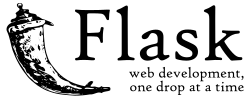
\includegraphics[width=6cm, height=3cm]{images/flask.png}
    \caption{Logo Flask}
\end{figure}

\noindent Flask est un micro-framework web pour Python. Dans notre architecture, nous l'avons utilisé pour créer des microservices d'intelligence artificielle qui s'intègrent avec notre API principale via des appels REST.

\subsubsection{Bibliothèques}

\noindent Pour enrichir les fonctionnalités de notre application, nous avons intégré plusieurs bibliothèques.

\paragraph{React}

\begin{figure}[H]
    \centering
    
\includegraphics[width=4cm, height=3cm]{images/react.png}
    \caption{Logo React}
\end{figure}

\noindent React est une bibliothèque JavaScript open-source pour créer des interfaces utilisateur. Nous l'avons utilisé pour développer notre interface utilisateur avec TypeScript, créant des composants réutilisables et une expérience utilisateur interactive.

\paragraph{Material UI (MUI)}

\begin{figure}[H]
    \centering
    
\includegraphics[width=3cm, height=3cm]{images/mui.png}
    \caption{Logo Material UI}
\end{figure}

\noindent Material UI \cite{mui} est une bibliothèque de composants React qui implémente le Material Design de Google. Nous l'avons utilisé pour créer une interface utilisateur cohérente et moderne, accélérant le développement avec ses composants pré-conçus.

\subsubsection{APIs}

\noindent Notre application intègre des services externes via des APIs pour étendre ses fonctionnalités.

\paragraph{Stripe API}

\begin{figure}[H]
    \centering
    
\includegraphics[width=3cm, height=3cm]{images/stripe.png}
    \caption{Logo Stripe}
\end{figure}

\noindent Stripe \cite{stripe} est une plateforme de paiement en ligne qui fournit des APIs pour traiter les paiements. Dans notre projet, nous avons intégré l'API Stripe pour gérer les transactions de paiement de manière sécurisée, permettant aux utilisateurs d'effectuer des achats directement dans l'application.

\section{Architecture de l'application}

\noindent Dans cette section, nous présentons l'architecture adoptée pour notre application, en détaillant l'organisation physique et logique de notre système.

\subsection{Architecture physique}

\noindent Notre application suit une architecture distribuée basée sur le modèle trois tiers, complétée par un service de traitement du langage naturel. Cette architecture garantit une séparation claire des responsabilités et une évolutivité optimale du système.

\noindent La figure 3.11 illustre l'organisation physique de notre application :

\begin{figure}[H]
    \centering
    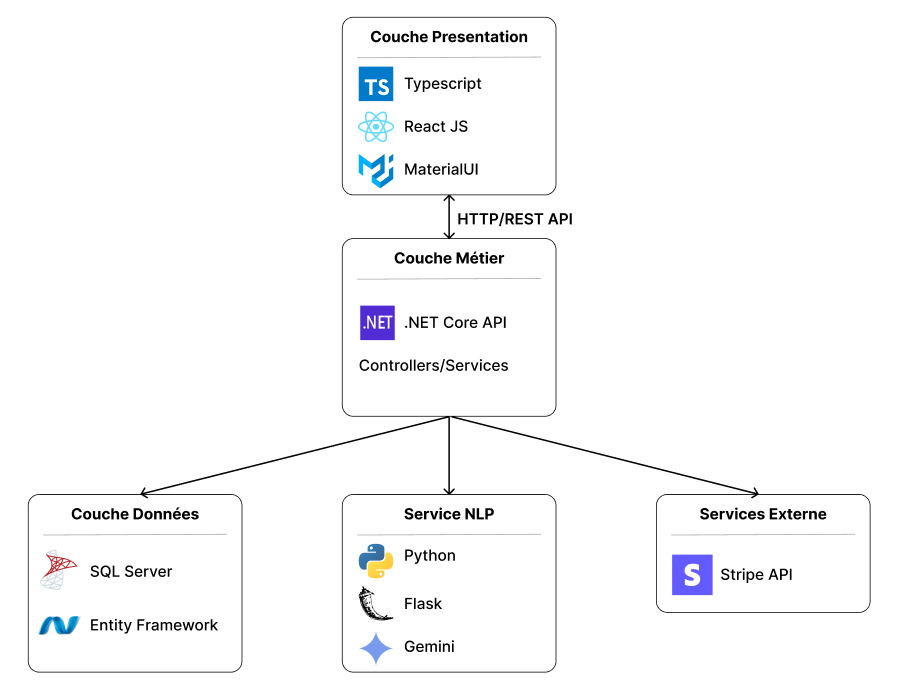
\includegraphics[width=16cm, height=13cm]{images/Architecturephysique.PNG}
    \label{fig:arch_physique}
    \caption{Architecture physique de l'application}
\end{figure}



\noindent\textbf{Couche Présentation} : Développée avec React et TypeScript, cette couche gère l'interface utilisateur et les interactions client. Elle utilise Material UI pour assurer une cohérence visuelle et communique avec la couche métier via des appels API REST.

\noindent \textbf{Couche Métier} : Implémentée avec .NET Core, cette couche centralise la logique applicative et orchestre les opérations entre les différentes couches. Elle expose des endpoints RESTful pour traiter les requêtes du frontend et coordonne les appels vers les services externes.

\noindent \textbf{Couche Données} : Basée sur SQL Server avec Entity Framework Core comme ORM, cette couche assure la persistance des données et gère toutes les opérations CRUD de l'application.

\noindent \textbf{Service NLP} : Service spécialisé développé en Python avec Flask, intégrant l'API Gemini de Google pour l'analyse des descriptions d'actions et la génération de recommandations intelligentes.

\noindent \textbf{Services Externes} : Intégration avec des APIs tierces comme Stripe pour le traitement des paiements, étendant les fonctionnalités de base de l'application.

\subsection{Architecture logique}

\noindent L'architecture logique de notre application repose sur le modèle MVC adapté aux technologies web modernes, complété par une approche microservices pour les fonctionnalités spécialisées.



\begin{figure}[H]
    \centering
    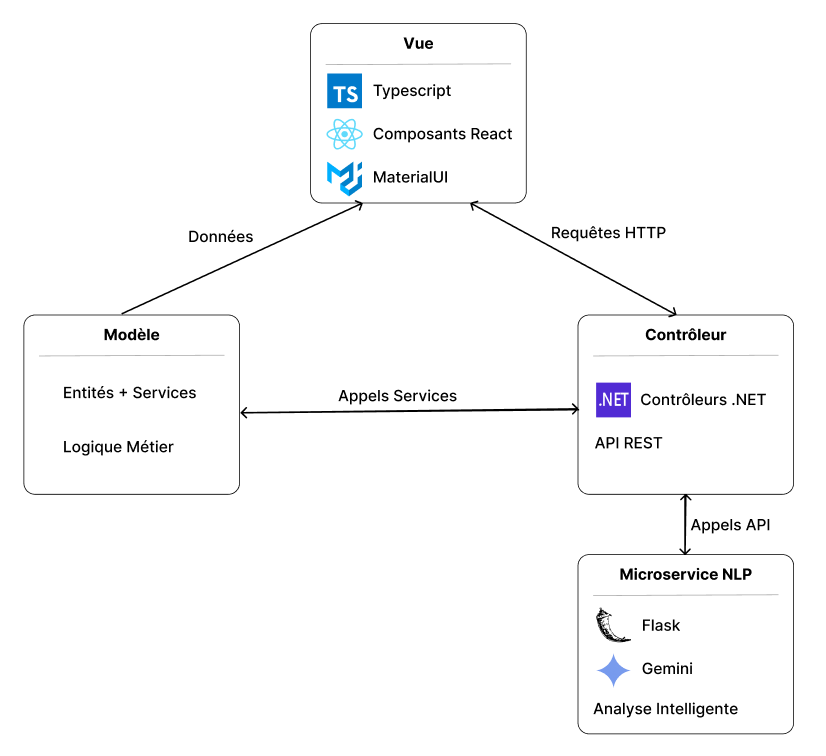
\includegraphics[width=15cm, height=13cm]{images/Architecturelogique.PNG}
    \label{fig:arch_logique}
    \caption{Architecture logique de l'application}
\end{figure}


\noindent \textbf{Modèle} : Représenté par les entités de données et les services métier de l'API .NET Core. Il encapsule la logique de traitement des données, les règles métier et les interactions avec la base de données via Entity Framework Core.

\noindent \textbf{Vue} : Constituée des composants React TypeScript qui gèrent l'affichage et les interactions utilisateur. Cette couche utilise Material UI pour maintenir une interface cohérente et responsive.

\noindent \textbf{Contrôleur (Controller)} : Implémenté par les contrôleurs .NET Core qui orchestrent les requêtes HTTP, valident les données d'entrée et coordonnent les appels entre les différentes couches et services.

\noindent \textbf{Architecture Microservices} : Le service NLP Flask fonctionne comme un microservice indépendant, communiquant avec l'API principale via des appels HTTP. Cette approche permet une évolutivité et une maintenabilité optimales des fonctionnalités d'intelligence artificielle.

\section*{Conclusion}

\noindent Ce chapitre a été consacré à la présentation des divers environnements de développement utilisés dans notre projet, ainsi qu'aux technologies employées pour la création de notre application web. Nous avons également abordé l'architecture N-tiers de notre système, illustrant comment les différentes couches interagissent pour fournir une solution complète et évolutive. Dans le prochain chapitre, nous procéderons à une analyse détaillée de la première release de notre projet.